\documentclass[french, titlepage, 11pt, a4paper]{article}
\usepackage{xunicode}
\usepackage{fontspec}
\usepackage[frenchb]{babel}
\usepackage{graphicx}
\usepackage{listings}
\usepackage[T1]{fontenc}
\usepackage{kpfonts}
\usepackage[usenames,dvipsnames]{color}



%\renewcommand*{\familydefault}{\sfdefault}

\renewcommand{\nobreakspace}{\nobreak\ }


\title{SUAPS}
\author{Clotilde \textsc{Massot} \and Alexandre \textsc{Garnier} \and Chimène Gaby \textsc{Nya Ngaha} \and Julien \textsc{Durillon}}

\begin{document}

%\maketitle
\begin{titlepage}

\begin{center}
    
\includegraphics[]{./logofac.png}\\[2cm]

    {\Large Interface Homme Machine}\\[2cm]

    {\Huge SUAPS\textcolor{red}{r} \textcolor{DarkOrchid}{beta}}\\[0.5cm]
    {\large \emph{Seeds of your success}}
\end{center}



\end{titlepage}


\fontsize{48}{48}
\fontspec{TeX Gyre Bonum Bold}
{\addfontfeature{Color=FF000099}W}\kern-1ex
{\addfontfeature{Color=0000FF99}S}\kern-0.8ex
{\addfontfeature{Color=DDBB2299}P}\kern-0.8ex
{\addfontfeature{Color=00BB3399}R}



\section{Analyse}
\label{sec:analyse}

	\subsection{Utilisateurs}
		La population des utilisateurs du point de vue du logiciel est
		sensiblement homogène: ce sont des utilisateurs de terminal android.
		Leur but est de se renseigner sur et de s'inscrire aux sports.

		Aucune connaissance du domaine n'est vraiment requise pour utiliser
		l'application.

	\subsection{Tâches}

	 Les tâches que l'utilisateur effectuera sont:

	    \paragraph{Parcours des sports}

	        Les sports sont classés par catégorie. Si on connaît le sport
	        cherché, l'accès à sa fiche se fait donc en 2 ou 3 \og clics\fg{}
	        maximum.

        \paragraph{Recherche de sport par critères}

            Pour un utilisateur cherchant à faire du sport en fonction de son
            emploi du temps: il pourra : rechercher par horaires, rechercher par
            lieu (contrainte géographique).

        \paragraph{Informations pratiques}

            Il est aussi possible de parcourir les lieux et d'en obtenir
            l'adresse ou le numéro.

        \paragraph{Inscription}

            La possibilité de s'inscrire à un sport peut aussi être proposée: il
            faut cependant passer par l'authentification inhérente à
            l'université.


    \subsection{Scénarii d'utilisation}

    Étant donné qu'il n'y a qu'une seule classe d'utilisateur, nous ne
    préciserons pas la classe effectuant chaque scénario.

        \paragraph{Accès à un sport}

            Dans ce cas, l'utilisateur lance l'application, choisit l'onglet
            Activités, choisit la catégorie voulue, puis sélectionne le sport.

            Il peut ensuite accéder à la fiche du lieu ou se déroule le sport, ou s'inscrire.

        \paragraph{Prospection par lieu}

            Dans ce scénario, l'utilisateur cherche un sport se déroulant dans un
            certain lieu. Il recherche donc dans la liste les lieux celui qui
            l'intéresse (on peut utiliser ici la géolocalisation pour avoir le
            lieu le plus proche). Une fois sur la fiche descriptive d'un lieu,
            on peut accéder aux sports qui s'y déroulent.

        \paragraph{Recherche par horaire}

            L'utilisateur va dans l'onglet \og Horaires\fg{} et entre ses vœux
            en terme de disponibilité. Les sports qui sont disponibles s'affichent.

\section{Conception de l'interface}

	Une fois définie la population des utilisateurs cible, vient la définition et
	la conception d'une interface efficace.
	Ici l'efficacité consiste en une solution à même d'offrir les fonctions
	attendues des utilisateurs dans une interface adaptée à leur connaissance de
	l'environnement applicatif.

	\subsection{Concept d'interaction}

	En celà, il s'agit ici de parvenir à proposer une solution simple et claire à
	utiliser, de telle sorte que l'accession aux fonctions clés de l'application
	soient accessibles rapidement et intuitivement.

	Dès lors, et afin de proposer une interface potentiellement connue de
	l'utilisateur, nous avons eu pour idée de s'inspirer de l'application AlloCiné
	pour Android.
	Notamment l'analogie entre la recherche et l'affichage de films d'un côté, de
	sports d'un autre, s'est imposée d'elle-même.

	\begin{figure}[ht]
		\centering
		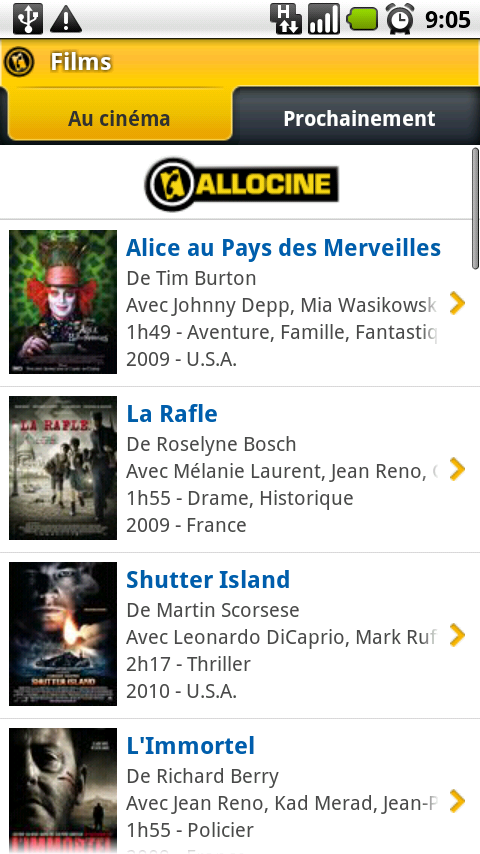
\includegraphics[width=0.5\textwidth]{allocine.png}
		\caption{Application AlloCiné: liste de films.}
		\label{fig:allocine}
	\end{figure}

	En outre, reprendre ainsi une interface que connaît l'utilisateur offre
	l'avantage de répondre à ses habitudes, automatismes et exigences.

	De la même manière, rendre l'accès aux fonctionnalités primordiales de
	l'applications accessibles en le moins d'actions possible est un objectif que
	nous nous sommes fixés.
	Dans cette optique, nous proposons un accès à ces fonctions dans un menu
	horizontal présent en haut de chaque écran.

	\subsection{Look and feel}

	Une sélection d'écran va ici être présentée afin d'illustrer la charte
	graphique adoptée, qu'il s'agisse de la disposition des diverses
	fonctionnalités que des images utilisées.

		\subsubsection{Écran d'accueil}

		\begin{figure}[ht]
			\centering
			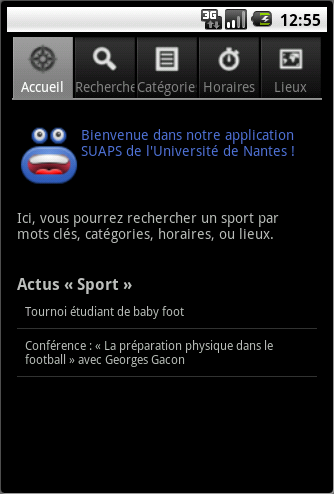
\includegraphics[width=0.5\textwidth]{accueil.png}
			\caption{Écran d'accueil de l'application}
			\label{fig:accueil}
		\end{figure}

		Lors du lancement de l'application, nous arrivons sur cet écran présentant
		succinctement les différentes fonctionnalités de l'application, que l'on
		retrouve donc en haut de l'écran, à savoir:

		\begin{itemize}
			\item la recherche de sports par nom;
			\item la prospection par catégorie;
			\item la recherche par horaires de disponibilité;
			\item l'affichage des lieux relatifs aux sports proposés par le SUAPS.
		\end{itemize}

		\subsubsection{Recherche par nom}

		\begin{figure}[ht]
			\centering
			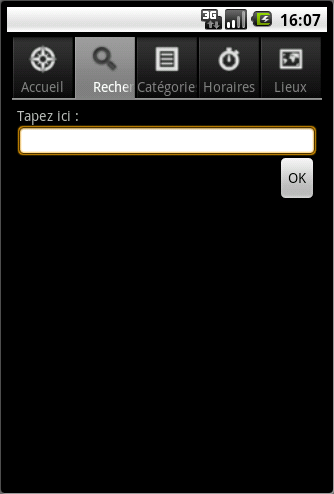
\includegraphics[width=0.5\textwidth]{recherche.png}
			\caption{Recherche par nom}
			\label{fig:recherche}
		\end{figure}

		Nous avons ici à faire à un simple champ où il s'agit d'entrer le nom du
		du sport à rechercher.

		\subsubsection{Prospection par catégorie}

		\begin{figure}[ht]
			\centering
			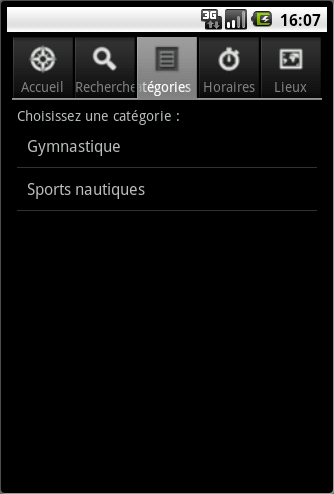
\includegraphics[width=0.5\textwidth]{categories.png}
			\caption{Catégories}
			\label{fig:categories}
		\end{figure}

		Ici seront listées les différentes catégories proposées par le SUAPS, la
		sélection d'une catégorie permettant ensuite l'affichage des sports
		correspondant à la dite catégorie.

		\subsubsection{Recherche par horaires}

		\begin{figure}[ht]
			\centering
			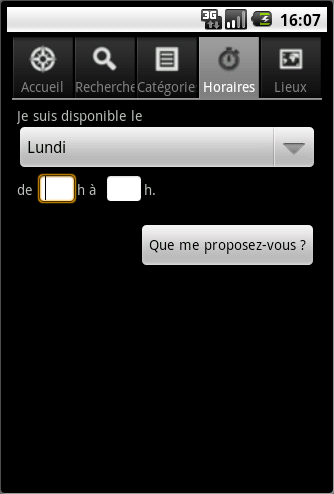
\includegraphics[width=0.5\textwidth]{horaires.png}
			\caption{Recherche par disponibilité}
			\label{fig:horaires}
		\end{figure}

		Cet écran permet à l'utilisateur de spécifier ses disponibilités afin de
		voir les sports auquel il peut dès lors participier durant ces périodes.

		Ainsi, la sélection d'un jour ouvrable et de l'intervalle horaire permet
		d'afficher les sports dispensés durant cette période.

	\subsection{Scénario d'utilisation: prospection d'un sport par lieu}

	Afin d'illustrer l'utilisation de l'application, nous proposons ici une suite
	d'actions et ses écrans intermédiaires permettant l'accès à un sport (ici le
	canoë-kayak).

	\begin{figure}[ht]
		\centering
		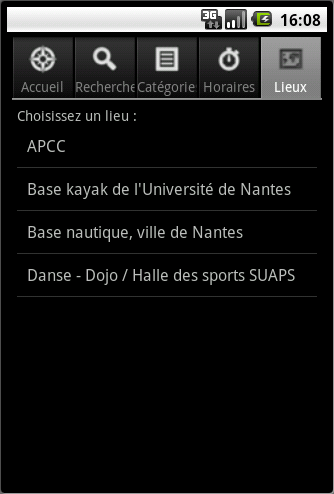
\includegraphics[width=0.5\textwidth]{lieux.png}
		\caption{Prospection par lieux}
		\label{fig:lieux}
	\end{figure}

	Dans un premier temps, l'écran de prospection par lieux (figure
	\ref{fig:lieux}) permet l'affichage des lieux où sont proposées des
	activités du SUAPS.

	\begin{figure}[ht]
		\centering
		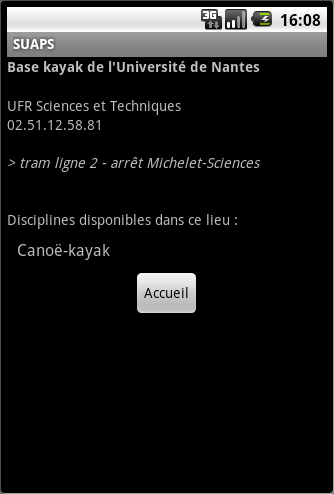
\includegraphics[width=0.5\textwidth]{basekayak.png}
		\caption{Base kayak de l'Université de Nantes}
		\label{fig:basekayak}
	\end{figure}

	Ensuite, la sélection d'un des lieux permet l'affichage des informations
	inhérentes, tel que le montre la figure \ref{fig:basekayak}.

	Notamment est affichée une liste des sports proposés en ce lieu.

	\begin{figure}[ht]
		\centering
		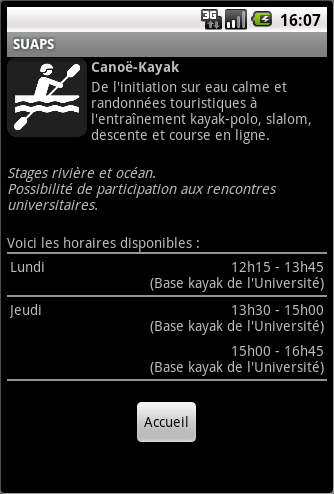
\includegraphics[width=0.5\textwidth]{canoekayak.png}
		\caption{Canoë-Kayak}
		\label{fig:canoekayak}
	\end{figure}

	Enfin, nous arrivons, via sélection d'un des sports au dernier écran, sur un
	écran présentant succinctement le sport considéré, ainsi que les horaires
	disponibles (figure \ref{fig:canoekayak}).

\section{Implémentation de l'application}

    Tout d'abord, l'application ne possède pas toutes les fonctionnalités prévue
    dans la section \ref{sec:analyse}. Notamment la partie inscription.


    La conception de l'application s'est faite en deux phases: création et accès
    à la base de données, et développement de l'interface.

    \subsection{Base de données}

        Pour le prototype réalisé, nous avons écrit les requêtes créant les
        tables et les remplissant au démarrage de l'application. Cela évite de
        devoir mettre un serveur à disposition et à y requêter les informations.

        Pour éviter un long démarrage de l'application, la base de données est
        remplie la première fois qu'on en a besoin.

        \paragraph{Bilan} N'ayant pas réussi à utiliser la base de donnée pour
        générer la liste des catégories et des activités, nous avons décidé de
        nous concentrer sur l'interface, et de faire des exemples en dur.


    \subsection{Interface étendue}

        Dans une version de production, il serait intéressant d'externaliser la
        base de données, et de fournir des services web pour récupérer les
        informations.

        L'intérêt d'externaliser la base est qu'en cas d'ajout ou de suppression
        d'informations, il n'y a pas besoin de fournir une nouvelle application.
        Un autre intérêt est justement de fournir une interface d'administration
        pour changer les informations relatives aux activités, catégories,
        lieux\dots

        Une coordination avec le SUAPS permettrait de fournir ces informations
        sur le site de l'université autant que dans l'application, en les centralisant.




\end{document}

